\chapter{Implementacja}
\label{cha:implementacja}

Zanim struktura aplikacji zostanie omówiona w większym detalu, należy opisać platformę, na której powstawała. W związku z faktem, iż implementacja jest pewnego rodzaju eskperymentem, 
od którego nie wymaga się produkcyjnej sprawności, zaimplementowano ją w języku programowania Ruby. Pozwala on na szybkie wdrażanie nowych funkcjonalności, jest w pełni obiektowym i
bardzo elastycznym językiem programowania. Jednak ponieważ Ruby jest językiem interpretowanym i posiada dynamiczne typowanie, zaawansowane możliwości metaprogramowania raz
zapewnia rozbudowane mechanizmy refleksji jego wydajność nie jest duża.
W związku z charakterystyką wybranej platformy program ma szanse działać poprawnie jedynie dla systemów typu Unix(Linux, OS X). Zastosowane zostały dwie wersje interepreterów Ruby'ego:
elementy 1. - 4. wymagają interpretera MRI, w wersji co najmniej 2.0.0. Jest to podstawowa implementacja tego języka, napisana w C, większość najważniejszych gemów(bibliotek) jest dostępna 
przede wszystkim dla tej dystrybucji. Natomiast moduły 5. - 8. wymagają użycia alternatywnej implementacji na JVM, o nazwie JRuby. Jest to wymaganie wykorzystywanej bazy grafowej Neo4j i dodatkowy powód,
dla którego podzielono aplikację na dwie części.

Aplikacja używa 3 baz danych: PostgreSQLa(\url{http://www.postgresql.org/}) do przechowywania ściągniętych stron, Neo4j(\url{http://www.neo4j.org/}) jako bazy grafowej i Redisa(\url{http://redis.io/})
 jako lekkiej bazy klucz - wartość. Wszystkie posiadają biblioteki umożliwiające interakcję z nimi na poziomie obiektów języka, co znacznie ułatwia projektowanie aplikacji. Również każda
 z technologii używanych w projekcie jest technologią \emph{Open Source}.

\section{Wymagania instalacyjne}
\label{sec:wymaganiaInst}

Aplikacja była rozwijana i testowana pod systemami typu Unix. Do instalacji i uruchomienia potrzebne są:
\begin{itemize}
\item system kontroli wersji Git (\url{http://git-scm.com/}),
\item Ruby zainstalowany za pomocą systemu kotroli wersji(preferowany rbenv - \url{http://rbenv.org/}),
\item Bundler (\url{http://bundler.io/}) i RubyGems (\url{http://rubygems.org/}),
\item serwer PostgreSQL,
\item baza grafowa Neo4j,
\item serwer Redis,
\item kolejka RabbitMQ.
\end{itemize}

Instrukcje instalacji, konfiguracji i uruchamiania poszczególnych komponentów znajdują się w dalszych częściach pracy.

\section{Implementacja komponentów 1. - 4.}

\subsection{Konfiguracja}
\label{subs:konfiguracjaMri}

Konfiguracja możliwa jest poprzez dwa pliki znajdujące się w katalogu \texttt{./config}: \texttt{database.yml} i \texttt{config.yml}. Umożliwiają one dostarczenie potrzebnych
informacji pozwalających na połączenie z relacyjną bazą danych, jak i na konfigurację zachowania aplikacji. Poniżej przedstawiony jest listing obu plików 
wraz z wyjaśnieniem dostępnych opcji.

\texttt{database.yml}

\begin{lstlisting}[frame=single]
defaults: &defaults
  adapter: postgresql
  encoding: unicode
  pool: 5
  username: user
  password: pass
  host: localhost

development:
  database: taskmaster_dev
  <<: *defaults
test:
  database: taskmaster_test
  <<: *defaults

\end{lstlisting}

Jest to plik instrumentujący używany w aplikacji ORM - \emph{Active Record}, w celu umożliwienia połączenia z bazą. Konieczne podanie jest typu(\emph{adapter}), 
użytkownika(\emph{user}), hasła(\emph{password}) i lokalizacji bazy(\emph{host}). Zdefiniowano również specjalne środowisko testowe, dostępne pod kluczem \texttt{test}.
Służy ono do definicji bazy powoływanej do egzystencji na czas testów, a następnie bezpowrotnie niszczonej. 
\newpage

\texttt{config.yml}

\lstset{language=ruby}
\begin{lstlisting}[frame=single]
crawler:
  connections: 20
  fetch_limit: 20
  url_pattern: '\/\/en\.wikipedia\.org\/wiki\/(?!\/|[A-Za-z]+:)'
  starting_page: 'http://en.wikipedia.org/wiki/Main_Page'
queue:
  limit: 50
logger:
  file: 'log/development.log'
  enabled: true

\end{lstlisting}

Plik ten przechowuje informacje konfiguracyjne aplikacji. Kolejno, odpowiadają one za:
\begin{itemize}
\item \texttt{crawler: connections} mówi, ile jednoczesnych asynchronicznych połączeń może wykonywać jeden proces robota.
\item \texttt{crawler: fetch\_limit} określa, ile na raz URLi jest wysyłanych do robota w celu ściągnięcia z Internetu. Nie jest t jednoznaczne z parametrem \texttt{connections}, 
w razie wysłania większej ilości adresów URL, niż jest otwieranych połączeń crawler wykona kilka iteracji i zwróci dokumenty odpowiadające wszystkim adresom.
\item \texttt{crawler: url\_pattern} przechowuje wyrażenie regularne, używane do filtracji adresów URL pobieranych ze stron. Jedynie adresy zgodne z wyrażeniem są zapamiętywane w bazie.
\item \texttt{crawler: starting\_page} podaje stronę startową, od której należy rozpocząć przeglądanie sieci.
\item \texttt{queue: limit} określa ile razy wywołana zostanie procedura przez kolejkę(ile stron zostanie wysłanych) przy jednym wywołaniu skryptu.
\item \texttt{logger: file} przechowuje relatywną wobec folderu projektu ścieżkę logowania.
\item \texttt{logger: enabled} to przełącznik, pozwalający na włąćzanie i wyłącznie loggera.
\end{itemize}

\subsection{Instalacja i uruchomienie}
\label{subs:instalacjaMri}

Po pobraniu repozytoruim i upewnieniu się, że pliki konfiguracyjne zawierają odpowiednie wartości, należy za pomocą \emph{shella} wykonać w katalogu z projektem następujące komendy:
\begin{enumerate}
\item \texttt{\$ bundle} - powoduje ściągnięcie wszystkich zależności,
\item \texttt{\$ rake db:create} - tworzy bazę,
\item \texttt{\$ PROJECT\_ENV=test rake db:create} -tworzy bazę testową,
\item \texttt{\$ rake db:migrate} - migruje bazę do scheme'y wymaganej przez aplikację.
\item \texttt{\$ PROJECT\_ENV=test rake db:migrate} - migruje bazę testową.
\item (opcjonalnie) \texttt{\$ rspec spec} w celu uruchomienia testów.
\end{enumerate}

Aby uruchomić robota internetowego należy w katalogu projektu wykonać polecenie
\texttt{\$ ./download}. W celu uruchomienia klienta kolejki RabbitMQ wystarczy w katalogu projektu wywołać \texttt{\$ ./publish}.
Aplikacja udostępnia również konsolę, umożliwiającą programiście interakcję z załadowanym środowiskiem. Aby z niej korzystać należy w katalogu projektu wywołać polecenie
\texttt{\$ ./console}. 
Zmienna środowiskowa \texttt{PRJOJECT\_ENV} używana jest do kontroli bazy danych, z którą łączy się aplikacja. Domyślnie przyjmuje ona wartość ``development'', a podczas testów
``test''. W celu uruchomienia np. konsoli z bazą testową, należy wywołać \texttt{\$ PROJECT\_ENV=test ./console}.

\section{Implementacja komponentów 5. - 8.}

\subsection{Konfiguracja}
\label{subs:konfiguracjaNeo4j}

Podobnie, jak opisana w sekcji \ref{subs:konfiguracjaMri} część projektu, również komponenty 5. - 8. są konfigurowane za pomocą pliku znajudującego się w katalogu 
\texttt{./config}: \texttt{config.yml}. Odpowiada on za przechowywanie informacji potrzebnych do połaczenia z bazami, lokalizacji plików z logami itd., jak i do 
ustalania parametrów silnika asocjacyjnego. Część opcji dotyczy również silnika symulacyjnego umożliwiającego przeprowadzanie eksperymentów z sieciami ANAKG, jednak
nie jest on bliżej omówiony w niniejszej pracy.

\lstset{language=ruby}
\begin{lstlisting}[frame=single]
payload:
  optional_limit: 2000
  min_word_length: 2
  max_word_length: 25
  max_sentence_length: 4

logger:
  enabled: true
  file: 'log/neo4ruby.log'

redis:
  host: '127.0.0.1'
  port: 6379

search_engine:
  simulation:
    alpha: 0.7
    beta: 0.8
    theta: 1.0
    initial_exc: 0.95
    max_iterations: 10
    min_change_rate: 0.2

  response_scanning:
    limit: 5
    levenshtein_max: 3
    # stopwords after http://www.webconfs.com/stop-words.php
    stopwords_file: 'data/stopwords'

  answer_resolving:
    limit: 10

experiment: 'exp1'

\end{lstlisting}
Poszczególne opcje odpowiadają za:
\begin{itemize}
\item \texttt{payload: optional\_limit} -  maksymalna ilość słów, która jest wprowadzana do bazy grafowej z pojedynczej sekwencji uczącej(pojedynczej strony).
\item \texttt{payload: min\_word\_length} - minimalna długość słowa(słowa krótsze są usuwane z sekwencji uczącej).
\item \texttt{payload: max\_word\_length} - maksymalna długość słowa, j.w.
\item \texttt{payload: max\_sentence\_length} - maksymalna długość zdania. Zdanie w aplikacji jest równoważne kontekstowi opisywanemu w rozdziale \ref{cha:budowaGrafu}.
\item \texttt{logger: enabled} - wł./wył. logowanie.
\item \texttt{logger: file} - lokalizacja pliku z logami.
\item \texttt{redis: } - dane potrzebne do połączenia z Redisem.
\item \texttt{search\_engine: } - parametry symulacji i asocjacyjnej wyszukiwarki internetowej.
\item \texttt{experiment: } - nazwa eksperymentu. Jest to \emph{de facto} ścieżka, w której przechowywane są pliki wbudowanej bazy grafowej. Zmieniając ją, zmienia się
bazę, z którą łączy się aplikacja.
\end{itemize}

\subsection{Instalacja i uruchomienie}
\label{subs:instalacjaMri}

Po pobraniu repozytorum i upewnieniu się, że pliki konfiguracyjne zawierają odpowiednie wartości, należy za pomocą \emph{shella} wykonać następujące komendy:
\begin{enumerate}
\item \texttt{\$ bundle} - powoduje ściągnięcie wszystkich zależności,
\item (opcjonalnie) \texttt{\$ rake test} w celu uruchomienia testów.
\end{enumerate}

Aby uruchomić serwer należy będąc w katalogu aplikacji wywołać polecenie \texttt{\$ ./start}. Przyjumje ono dwa opcjonalne argumenty: \texttt{-e -\--experiment EXP\_NAME} daje możliwość
ręcznego ustawienia bazy, z którą łączy się aplikacja. Zmienna ustawiona w ten sposób nadpisze konfigurację zapisaną w pliku; \texttt{-q -\--queue QUEUE\_NAME} pozwala na zmianę nazwy
kolejki, na której nasłuchuje serwer. Należy jednak wspomnieć, iż ustawienia te były wykorzystywane głównie do rozwoju aplikacji na jej wczesnym stadium, docelowo wszystkie ustawienia
zostaną przeniesione do pliku konfiguracyjnego.

Aplikacja posiada również skrypt ładujący całe środowisko i pozwalający na interaktywną jego eksplorację za pomocą linii komand. Uruchamiany jest on poleceniem \texttt{./console} z
folderu projektu. W razie, gdy istnieje potrzeba połączenia się z inną bazą, niż wyszczególniona w pliku konfiguracyjnym, można użyć opcji \texttt{-e -\--experiment EXP\_NAME}.

\subsection{Struktura przechowywanych informacji}
\label{subs:struktNeo4j}

Z powodów wydajnościowych zdecydowano się na użycie dwóch rodzajów baz: Neo4j odpowiada za przechowywanie struktury grafu,
jego trawersowanie i integralność. To rozwiązanie stosowane jest ze względu na przyjazne API i łatwość integracji z aplikacją. Jednak ze wzgledu na duża ilość wpisów do bazy
podczas tworzenia struktury grafu AGDS(docelowo setki tysięcy stron) oraz konieczność sekwencyjnego budowania grafu, atrybuty elementów grafu, takie jak np. słowa wchodzące
w skład sekwencji uczącej, czy wagi krawędzi sa przechowywane przez prawie cały czas w pamięci programu i zapisywane okresowo w Redisie. Dzięki temu ograniczono znacząco ilość
kosztownych operacji I/O.

\begin{figure}[h!]
    \label{graph:logic_graph}
    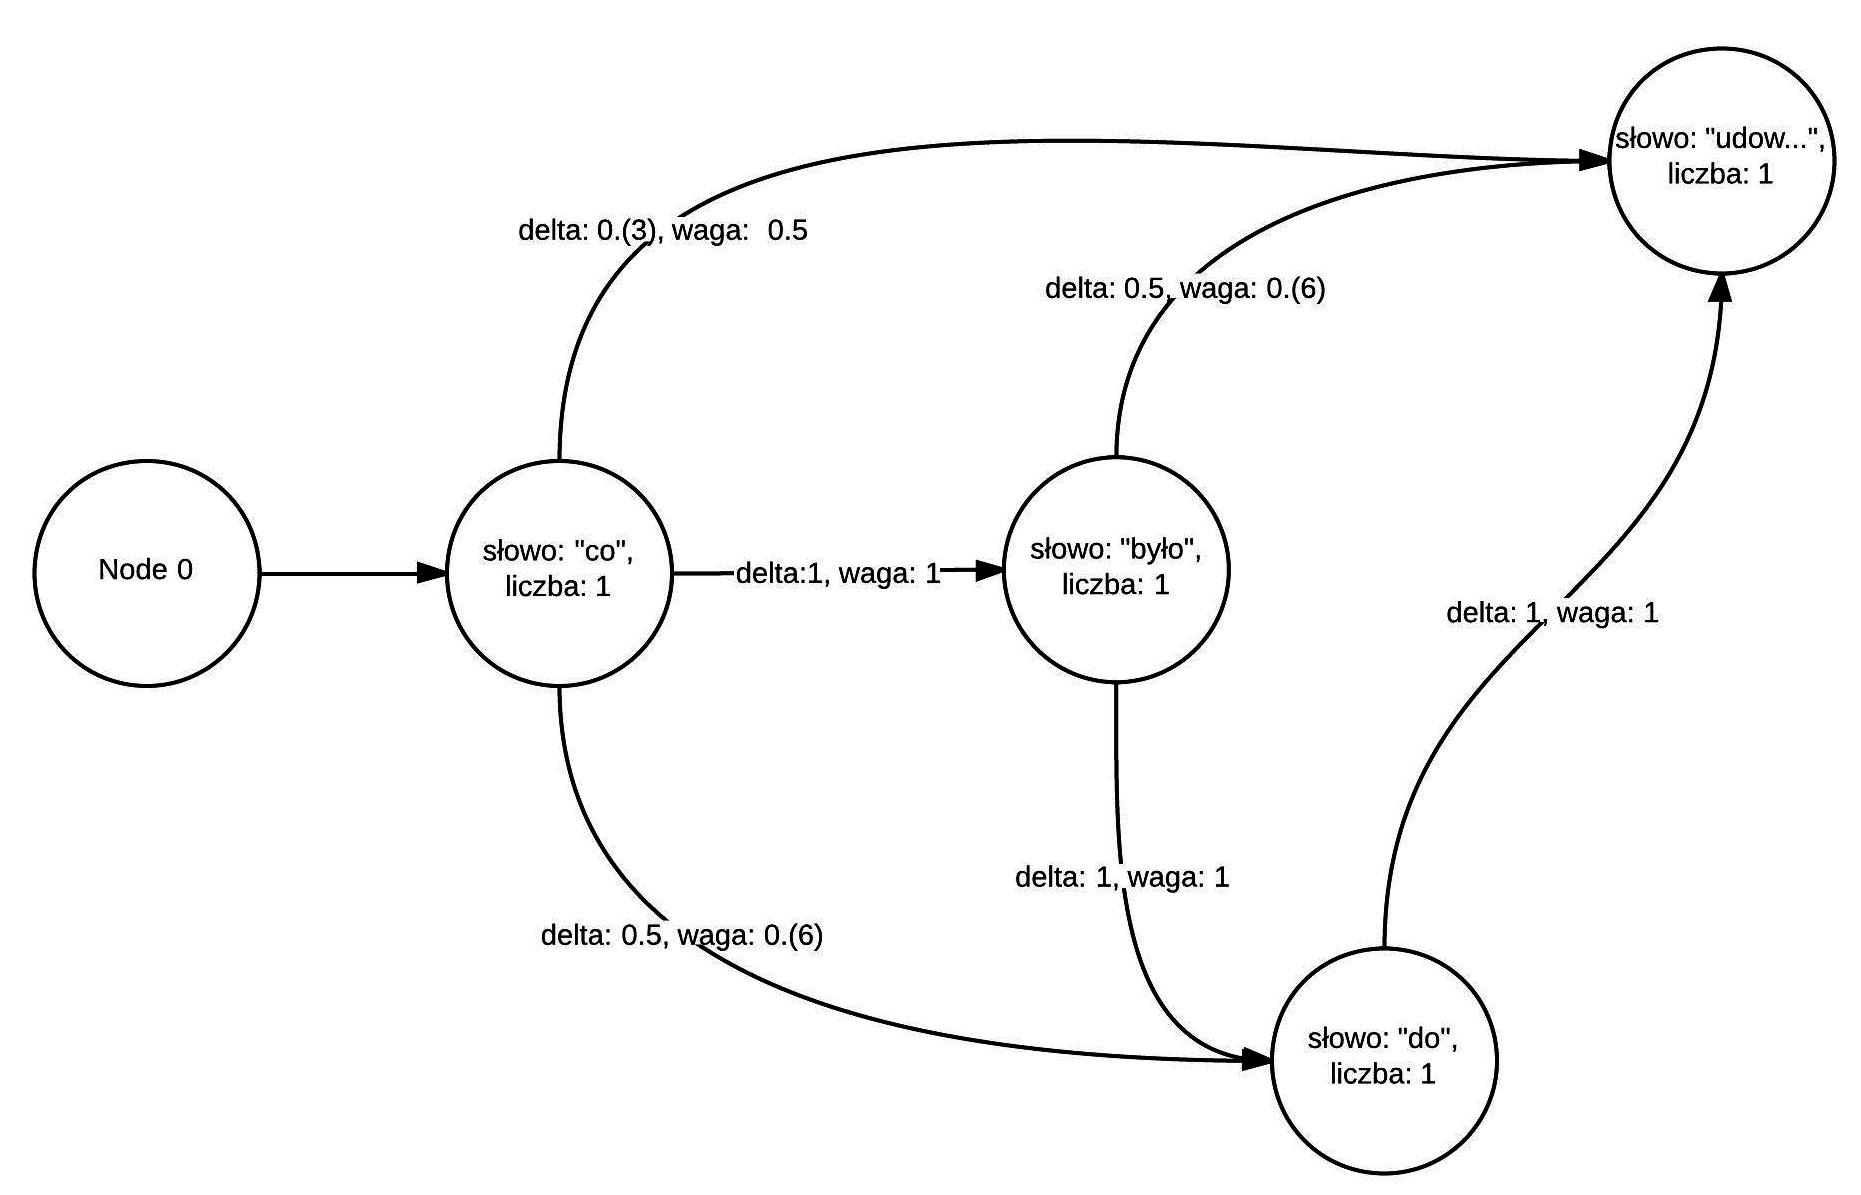
\includegraphics[width=\textwidth]{logic_graph}
    \caption{Przykład reprezentacji sekwencji uczącej w bazie grafowej.}
\end{figure}

Na rysunku \ref{graph:logic_graph} przedstawiona jest logiczna struktura grafu, widziana przez komponenty 5. - 7. Jest to struktura AGDS, powstała na podstawie sekwencji uczącej
$S = \{co, byl{}o, do, udow...\}$. Widoczny jest również domyślny węzeł zerowy(Node 0), obecny w każdej strukturze Neo4j.
